\documentclass[conference]{IEEEtran}
\IEEEoverridecommandlockouts
% The preceding line is only needed to identify funding in the first footnote. If that is unneeded, please comment it out.
\usepackage{cite}
\usepackage{amsmath,amssymb,amsfonts}
\usepackage{algorithmic}
\usepackage{graphicx}
\usepackage{textcomp}
\usepackage{xcolor}
\usepackage{listings}
\usepackage{acronym}
\usepackage{listing-style}
\usepackage{subcaption}
\usepackage{tikz}
\usetikzlibrary{arrows,shapes.geometric,positioning,automata,calc}
\usepackage[hidelinks]{hyperref}
\usepackage[inline]{enumitem}
\usepackage{siunitx}
\DeclareSIUnit{\decibelmeter}{dBm}
\providecommand{\decibel}{dB}
\providecommand{\decibelmeter}{dBm}
\providecommand{\qty}[2]{#1#2}


\acrodef{api}[API]{application-program interface}
\acrodef{dsl}[DSL]{domain-specific language}
\acrodef{iot}[IoT]{Internet of Things}
\acrodef{cas}[CAS]{collective adaptive system}
\acrodef{qos}[QoS]{quality of service}
\acrodef{rssi}[RSSI]{received signal strength indicator}
\acrodef{poi}[PoI]{point of interest}

\usepackage{cleveref}
\usepackage{color}
\usepackage{nicefrac}
\usepackage{wasysym}


\lstdefinelanguage{pulv}[]{Kotlin}{
%  basicstyle=\small\ttfamily\lst@ifdisplaystyle\footnotesize\fi,
%	frame=single,
%	escapechar=\%,
%  keywordstyle=\color{blue},
  keywordstyle=[3]\bfseries{},
  keywords=[3]{pulverizedSystem,device,and,deployableOn,pulverizationRuntime,startsOn,onDevice,reconfigurationRules,reconfigures,movesTo},
%  emph={DeviceBehaviour,DeviceCommunication,DeviceSensors,DeviceActuators,HighLoad,LowBattery},
%  sensitive=true,
%  morecomment=[l]{//},
%  morecomment=[n]{/*}{*/},
%  commentstyle=\color{green!40!black},
%  morestring=[b]",
%  morestring=[b]',
%  morestring=[b]""",
%  stringstyle=\ttfamily\color{orange},
}
\lstset{language=pulv,
basewidth=0.555em % decreases spacing between chars
}


\def\BibTeX{{\rm B\kern-.05em{\sc i\kern-.025em b}\kern-.08em
    T\kern-.1667em\lower.7ex\hbox{E}\kern-.125emX}}
    
\newcommand{\meta}[1]{{\color{blue}#1}}   

\lstset{xleftmargin=0.3cm,numbersep=5pt} 

\makeatletter
\newcommand{\linebreakand}{
  \end{@IEEEauthorhalign}
  \hfill\mbox{}\par
  \mbox{}\hfill\begin{@IEEEauthorhalign}
}
\makeatother

    
\begin{document}

\title{Declarative Deployment Reconfiguration of Pulverised Collective Adaptive Systems at Runtime
\thanks{
    This work has been supported by the Italian PRIN Project COMMON-WEARS (2020HCWWLP) and the EU/MUR FSE REACT-EU PON R\&I 2014-2020.
}
}

\author{\IEEEauthorblockN{1\textsuperscript{st} Danilo Pianini}
\IEEEauthorblockA{\textit{Department of Computer Science and Engineering} \\
\textit{Alma Mater Studiorum---Università di Bologna}\\
Cesena, Italy \\
danilo.pianini@unibo.it}
\and
\IEEEauthorblockN{2\textsuperscript{nd} Roberto Casadei}
\IEEEauthorblockA{\textit{Department of Computer Science and Engineering} \\
\textit{Alma Mater Studiorum---Università di Bologna}\\
Cesena, Italy \\
roby.casadei@unibo.it}
\linebreakand
\IEEEauthorblockN{3\textsuperscript{rd} Nicolas Farabegoli}
\IEEEauthorblockA{\textit{Department of Computer Science and Engineering} \\
\textit{Alma Mater Studiorum---Università di Bologna}\\
Cesena, Italy \\
nicolas.farabegoli@unibo.it}
\and
\IEEEauthorblockN{4\textsuperscript{th} Mirko Viroli}
\IEEEauthorblockA{\textit{Department of Computer Science and Engineering} \\
\textit{Alma Mater Studiorum---Università di Bologna}\\
Cesena, Italy \\
mirko.viroli@unibo.it}
}

\maketitle

\begin{abstract}
In recent years,
the infrastructure supporting the execution of situated distributed computations
evolved at a fast pace.
%
Modern collective adaptive applications -- as found in the Internet of Things, swarm robotics, and social computing -- are designed to be executed on very diverse devices
and to be deployed on infrastructures composed of devices ranging from cloud servers to wearable devices,
constituting together a cloud-edge continuum.
%
The availability of such an infrastructure opens to better resource utilisation and performance
but, contextually, introduces new challenges to software designers,
as applications must be conceived to be able to adapt their deployment to changing deployment domains and conditions.
%
In this paper,
we introduce a practical framework for the development of collective adaptive systems
based on the concept of \emph{pulverisation},
meant to neatly separate business logic and deployment concerns,
allowing applications to be defined independently of the infrastructure they will execute upon.
%
The framework is based on a domain-specific language capturing,
in a declarative fashion,
pulverised application components, device capabilities, resource allocation, and (runtime re-) configuration policies.
%
The framework, implemented in Kotlin multiplatform and available as open source,
is then evaluated in a small-scale real-world demo and in a city-scale simulated scenario,
demonstrating the feasibility of the approach
and its potential benefits in achieving better trade-offs between performance and resource utilisation.
\end{abstract}

\begin{IEEEkeywords}
runtime reconfiguration, distributed systems, self-adaptation, self-organisation, pulverisation, deployment.
\end{IEEEkeywords}

\acrodef{ourframework}[\textsc{PulvReAKt}]{Pulverisation with Reconfigurable Adaption in Kotlin}
\newcommand{\ourframework}{\ac{ourframework}}

%\meta{LIMIT 10 pages incl. refs; DEADLINE 19 may}

\section{Introduction}\label{sec:introduction}

Recent technological and scientific advances
 are extending 
 both the \emph{kinds of applications and systems} that are being addressed  
 as well as their \emph{supporting infrastructure}~\cite{DBLP:journals/iot/GillXOPBSGSWASM22}.
%
Emerging applications
 are, for instance, those based on \emph{\acp{cas}}~\cite{DBLP:journals/computer/Abowd16,DBLP:journals/sttt/NicolaJW20},
 namely collections of devices and agents
 that interact to solve problems or provide services while adapting \emph{as a whole} to dynamic environments.
%
Examples include 
  \ac{iot} deployments, 
  swarms of robots,
  social computing systems,
  crowds of wearable-augmented people, and so on---supporting activities like monitoring,
  transportation, coordination, and other forms of collective intelligence~\cite{casadei2023artl-ci}.
%
Regarding infrastructure,
 it is mounting the idea of the \emph{cloud-edge continuum}~\cite{DBLP:journals/iot/BittencourtISFM18}: 
a multi-layer heterogeneous network of devices (ranging from large and powerful cloud servers to small connected \emph{things})
on which software can compute, store, and exchange data in a distributed fashion, while 
optimising for performance and resource utilisation.
%

This kind of infrastructure is also valuable for  \acp{cas}~\cite{DBLP:journals/tpds/HongCHGZ19,DBLP:journals/comsur/WangZZMLW20,DBLP:journals/comsur/AfrinJRRWH21,IEEE-IoTJ-pulverization-simulation},
which generally feature components that,
depending on the conditions at hand,
could benefit from being deployed on different devices or from \emph{offloading} some of their  tasks.
%
However, exploiting this infrastructure,
 poses new challenges to \ac{cas} application designers.
%
Commonly, in fact, applications are designed with a specific infrastructure in mind,
whose assumptions unavoidably leak into the application logic~\cite{Spolsky2004},
unless captured and encapsulated away from it:
the higher the coupling between the application and the infrastructure,
the harder it is for the former to exploit the latter's full potential and adapt to changes.

The general solution is to devise 
 a reasonable \emph{partitioning}~\cite{DBLP:journals/jnca/LiuASGBQ15} of the software system
 and a corresponding (dynamic) deployment plan 
 defining the mapping between the software components and the target deployment domain~\cite{DBLP:journals/jss/ArcangeliBL15}.
%
In the context of \acp{cas},
 previous work proposes an application partitioning schema,
 called \emph{pulverisation}~\cite{FI2020-pulverization},
 the fosters the decoupling of business logic and deployment concerns.
%
In short, the core idea is to consider devices as \emph{logical} entities,
whose software can be designed as (or broken down to, if already existing) an ensemble of \emph{five components
(behaviour, state, communication, sensors, and actuators)}
 that can be deployed with flexibility on available infrastructure without (ideally) affecting application functionality. %whose actual host can be decided at deployment time.
%
This way, the designer can focus on the business logic at hand,
delaying an optimised deployment to later stages of the sofware design,
thus gaining resilience to changes in the infrastructure or in non-functional requirements.
%
One limitation of previous work on pulverisation regards dynamicity:
although the application can be deployed on arbitrary systems,
there is no support for the reconfiguration of components at runtime, as a reaction to changing conditions or requirements.

In this work,
we continue the research on pulverised systems by providing two key contributions:
\textbf{first}, we extend the theoretical framework of pulverisation by adding support for
\emph{runtime configuration rules}, allowing pulverised components to move at runtime across different hosts;
\textbf{second}, we provide a practical implementation in Kotlin called \emph{\ourframework{}} which,
to the best of our knowledge,
is the first \emph{practical framework supporting pulverisation}. % for a general-purpose language.
%
To evaluate \ourframework{}, we exercise it through two case studies:
a small-scale real-wold demonstration, and a city-scale simulated scenario.

%\meta{
%\begin{itemize}
%    \item need for deployment-independent specs
%    \item need for runtime reconfiguration (achieve \ac{qos} in face of changing conditions --- green computing?)
%    \item declarativity over imperative approaches (note: can be compared with the trend in general softeng/build systems)
%\end{itemize}
%}

The manuscript is organised as follows.
%
\Cref{sec:background} provides background on deployment and pulverisation.
%
\Cref{sec:contribution} describes the proposed \ac{dsl} and platform.
%
\Cref{sec:evaluation} provides an evaluation of the approach.
%
\Cref{sec:rw} covers related work.
%
Finally, \Cref{sec:conclusion} concludes the paper and highlights directions for future work.

\section{Background}\label{sec:background}

\subsection{Deployment and Reconfiguration: Basic Concepts}\label{sec:background:dep}

The \emph{deployment view} is a well-known architectural viewpoint for software systems,
concerned with the mapping of \emph{software components} to \emph{physical machines}~\cite{DBLP:journals/software/Kruchten95}, 
 and supported by modelling notations like \emph{UML Deployment diagrams}.
%
Here, we provide a brief introduction to deployment and reconfiguration, based on the conceptual characterisation of~\cite{DBLP:journals/jss/ArcangeliBL15,carzaniga1998characterization}.
%
A \emph{site} is a set of computers (\emph{hosts}) that may host a \emph{software system}, i.e., a product described by a coherent collection of artefacts and consisting of a set of \emph{deployment units} that can be independently operated.
%
\emph{(Software) Deployment} is the process of moving and making a software system available and operational from one or more \emph{producer sites} to a target set of \emph{consumer sites}, also called the \emph{deployment domain}.
%
The \emph{deployment plan} defines 
 the mapping between the software system
 and the deployment domain,
 possibly augmented with further information (e.g., metadata, constraints, preferences).
%
Common deployment-related activities 
 include: (i) \emph{release/update} of the software system at the producer site;
 (ii) \emph{installation/deinstallation} at/from the consumer sites;
 (iii) \emph{activation/deactivation}, for starting/stopping the components;
 (iv) \emph{reorganisation} of the software system;
 and (v) \emph{redistribution}, i.e., changing the deployment plan.
%
According to the analytical framework of~\cite{DBLP:journals/jss/ArcangeliBL15},
  the problem of (automatic) deployment of distributed software system can be addressed by considering
 (i) the nature of the software to be deployed (e.g., how the software system is split into components);
 (ii) the nature of the deployment domain (i.e. the characteristics and topology of the available infrastructure);
 (iii) how the deployment is designed (e.g., how the deployment plan is specified);
 and 
 (iv) how the deployment is performed (e.g., how deployment activities are carried out).
%
By an operational point of view, 
 deployment may be supported by a so-called \emph{runtime} or \emph{middleware}~\cite{DBLP:journals/cacm/GazisK22}.
%
Related work covering these issues is provided in \Cref{sec:rw}.
%
In the following, we introduce the deployment approach 
  that we extend and upon which we develop \ourframework{}.



\begin{figure}
\tikzset{-,
  host/.style={rectangle,draw,line width={2pt},inner sep=10pt,
  	outer sep=0, minimum height=1.5cm, minimum width=1.8cm, %text height=0.2cm, 
  	text depth=0.5cm,
  	fill=black!10!white
  },
  node/.style={rectangle,draw,dotted,line width={1pt}, inner sep=2pt, 
  	fill=blue!20!white,
  	font=\large
  },
  nodeA/.style={node,fill=red!20!white},
  nodeB/.style={node,fill=green!20!white},
  nodeC/.style={node,fill=black!30!white},
  nodeD/.style={node,fill=white!20!white},
  plink/.style={line width=2pt},
  llink/.style={dotted,line width=2pt,red},
  hostThin/.style={rectangle,draw,line width={0.5pt},inner sep=10pt,
  	outer sep=0, minimum height=1.1cm, minimum width=1.8cm, %text height=0.2cm, 
  	text depth=0.5cm,
  	fill=black!10!white
  },
  lnode/.style={node,minimum width=0.55cm,minimum height=0.55cm},
  loglink/.style={->,line width=1.5pt}
}
\def\nm{0.35cm} %nm = node margin offset
\def\tpscale{0.7}
\newcommand{\agent}{device}
\newcommand{\LSens}{\boldsymbol{\sigma}}
\newcommand{\LComp}{\boldsymbol{\beta}}
\newcommand{\LComm}{\boldsymbol{\chi}}
\newcommand{\LAct}{\boldsymbol{\alpha}}
\newcommand{\LState}{\boldsymbol{\kappa}}

\begin{minipage}{\columnwidth}
\centering
\begin{tikzpicture}[every node/.style={scale=1}]
\node[hostThin,minimum width=3.4cm,minimum height=3cm,dashed]
 (h1) [label={[yshift=0.35cm]above:{\textbf{logical \agent{}}}}] {};

\node[lnode] (d1) at (h1.north west) [xshift=\nm,yshift=-\nm,label=above:{behaviour}] {$\LComp$};
\node[lnode] (d2) at (h1.north east) [xshift=-\nm,yshift=-\nm,label=above:{communication}] {$\LComm$};
\node[lnode] (d3) at (h1.center) [xshift=0,yshift=0,label=right:{state/knowledge}] {$\LState$};
\node[lnode] (d4) at (h1.south west) [xshift=\nm,yshift=\nm,label=below:{sensors}] {$\LSens$};
\node[lnode] (d5) at (h1.south east) [xshift=-\nm,yshift=\nm,label=below:{actuators}] {$\LAct$};

\node[hostThin,minimum width=2.3cm,minimum height=2.3cm,dashed]
 (h2) [right=2cm of h1, label={above:{\textbf{neighbour \agent{}}}}] {};

\node[lnode] (d21) at (h2.north west) [xshift=\nm,yshift=-\nm] {$\LComm$};
\node[lnode] (d22) at (h2.north east) [xshift=-\nm,yshift=-\nm] {$\LComp$};
\node[lnode] (d23) at (h2.center) [xshift=0,yshift=0] {$\LState$};
\node[lnode] (d24) at (h2.south west) [xshift=\nm,yshift=\nm] {$\LSens$};
\node[lnode] (d25) at (h2.south east) [xshift=-\nm,yshift=\nm] {$\LAct$};

\draw[loglink] (d1) -- (d3);
\draw[loglink] (d2) -- (d3);
\draw[loglink] (d3) -- (d1);
\draw[loglink] (d3) -- (d2);
\draw[loglink] (d4) -- (d3);
\draw[loglink] (d3) -- (d5);

\draw[loglink] (d21) -- (d23);
\draw[loglink] (d22) -- (d23);
\draw[loglink] (d23) -- (d21);
\draw[loglink] (d23) -- (d22);
\draw[loglink] (d24) -- (d23);
\draw[loglink] (d23) -- (d25);

\draw[loglink] (d2.east) -- (d21.west);
\draw[loglink] (d21.west) -- (d2.east);


\end{tikzpicture}
\subcaption{A logical device, split into sub-components, and one of its neighbours.\label{fig:pulv:dev}}
\end{minipage}
\\[0.2cm]
\begin{minipage}{\columnwidth}
\def\nm{0.3cm} %nm = node margin offset

\begin{minipage}{0.48\columnwidth}\centering
\begin{tikzpicture}[node distance=1.0cm and 0.5cm,every node/.style={scale=\tpscale}]
% physical nodes
\node[host] (h1) [anchor=north,label=above:{}] {};
\node[host] (h2) [right=of h1,label=above:{}] {};
\node[host] (h3) [below=of h1, label=above:{}] {};
\node[host] (h4) [right=of h3, label=above:{}] {};

\node[node] (n11) at (h1.south west) [xshift=\nm,yshift=\nm] {$\LSens$};
\node[node] (n12) at (h1.south east) [xshift=-\nm,yshift=\nm] {$\LComm$};
\node[node] (n13) at (h1.north east) [xshift=-\nm,yshift=-\nm] {$\LAct$};
\node[node] (n14) at (h1.north west) [xshift=\nm,yshift=-\nm] {$\LComp$};
\node[node] (n15) at (h1) [] {$\LState$};
% logical node 2
\node[nodeA] (n21) at (h2.south west) [xshift=\nm,yshift=\nm] {$\LComm$};
\node[nodeA] (n22) at (h2.south east) [xshift=-\nm,yshift=\nm] {$\LAct$};
\node[nodeA] (n23) at (h2.north east) [xshift=-\nm,yshift=-\nm] {$\LSens$};
\node[nodeA] (n24) at (h2.north west) [xshift=\nm,yshift=-\nm] {$\LComp$};
\node[nodeA] (n25) at (h2) [] {$\LState$};
% logical node 3
\node[nodeB] (n31) at (h3.south west) [xshift=\nm,yshift=\nm] {$\LSens$};
\node[nodeB] (n32) at (h3.south east) [xshift=-\nm,yshift=\nm] {$\LAct$};
\node[nodeB] (n33) at (h3.north east) [xshift=-\nm,yshift=-\nm] {$\LComm$};
\node[nodeB] (n34) at (h3.north west) [xshift=\nm,yshift=-\nm] {$\LComp$};
\node[nodeB] (n35) at (h3) [] {$\LState$};
% logical node 4
\node[nodeC] (n41) at (h4.south west) [xshift=\nm,yshift=\nm] {$\LSens$};
\node[nodeC] (n42) at (h4.south east) [xshift=-\nm,yshift=\nm] {$\LAct$};
\node[nodeC] (n43) at (h4.north east) [xshift=-\nm,yshift=-\nm] {$\LComp$};
\node[nodeC] (n44) at (h4.north west) [xshift=\nm,yshift=-\nm] {$\LComm$};
\node[nodeC] (n45) at (h4) [] {$\LState$};

% physical links
\draw[plink] 
	(h1) -- (h2)
	(h2) -- (h3)
	(h2) -- (h4)
	(h3) -- (h4)
;
% logical links
\draw[llink]
    (n12) to [] (n21)
    (n21) to [] (n44)
    (n21) to [bend right=30] (n33)
    (n33) to [] (n44);
\end{tikzpicture}
\subcaption{Peer-to-peer architecture: one-to-one mapping between logical and physical devices, with no offloading.\label{fig:pulv:p2p}}
\end{minipage}
%\hfill
%\begin{minipage}{0.48\columnwidth}\centering
%\begin{tikzpicture}[node distance=1.0cm and 0.5cm,
%every node/.style={scale=\tpscale}]
%
%% physical nodes
%\node[host,minimum width=1.5cm] (h1) [anchor=north,label=above:{}] {};
%\node[host,minimum width=1.5cm] (h2) [right=of h1,label=above:{}] {};
%\node[host,minimum width=1.5cm] (h3) [right=of h2, label=above:{}] {};
%\node[host,minimum width=2.5cm] (he) [above right=0.6cm and -1cm of h1,label=above:{}] {};
%\node[host,minimum width=3.5cm] (h5) [above=2.6cm of h2,label=right:{}] {};
%
%\node[node] (n11) at (h1.south west) [xshift=\nm,yshift=\nm] {$\LSens$};
%\node[node] (n12) at (h1.south east) [xshift=-\nm,yshift=\nm] {$\LAct$};
%\node[node] (n13) at (h1.north east) [xshift=-\nm,yshift=-\nm] {$\LState$};
%\node[node] (n14) at (h1.north west) [xshift=\nm,yshift=-\nm] {$\LComp$};
%\node[node] (n15) at (he) [xshift=-2*\nm] {$\LComm$};
%% logical node 2
%\node[nodeA] (n21) at (h2.south west) [xshift=\nm,yshift=\nm] {$\LSens$};
%\node[nodeA] (n22) at (h2.south east) [xshift=-\nm,yshift=\nm] {$\LAct$};
%\node[nodeA] (n23) at (h2.north east) [xshift=-\nm,yshift=-\nm] {$\LState$};
%\node[nodeA] (n24) at (h2.north west) [xshift=\nm,yshift=-\nm] {$\LComp$};
%\node[nodeA] (n25) at (he) [xshift=0] {$\LComm$};
%% logical node 3
%\node[nodeB] (n31) at (h3.south west) [xshift=\nm,yshift=\nm] {$\LSens$};
%\node[nodeB] (n32) at (h3.south east) [xshift=-\nm,yshift=\nm] {$\LAct$};
%\node[nodeB] (n33) at (h3.north east) [xshift=-\nm,yshift=-\nm] {$\LState$};
%\node[nodeB] (n34) at (h3.north west) [xshift=\nm,yshift=-\nm] {$\LComp$};
%\node[nodeB] (n35) at (h5) [xshift=2*\nm] {$\LComm$};
%
%% physical links
%\draw[plink] 
%	(h1) -- (he)
%	(h2) -- (he)
%	(h3) -- (h5)
%	(he) -- (h5);
%
%\draw[llink]
%    %(n15) to [bend left=20] (n35)
%    (n25) to [bend left=30] (n35);
%\end{tikzpicture}
%\subcaption{Communication component offloaded.\label{fig:pulv:comm}}
%\end{minipage}
%\\[0.2cm]
%\begin{minipage}{0.48\columnwidth}\centering
%\begin{tikzpicture}[node distance=1.0cm and 0.5cm,
%every node/.style={scale=\tpscale}]
%
%% physical nodes
%\node[host,minimum width=1.5cm] (h1) [anchor=north,label=above:{}] {};
%\node[host,minimum width=1.5cm] (h2) [right=of h1,label=above:{}] {};
%\node[host,minimum width=1.5cm] (h3) [right=of h2, label=above:{}] {};
%\node[host,minimum width=2.5cm] (he) [above right=0.6cm and -1cm of h1,label=above:{}] {};
%\node[host,minimum width=3.5cm] (h5) [above=2.6cm of h2,label=right:{}] {};
%
%\node[node] (n11) at (h1.south west) [xshift=\nm,yshift=\nm] {$\LSens$};
%\node[node] (n12) at (h1.south east) [xshift=-\nm,yshift=\nm] {$\LAct$};
%\node[node] (n13) at (he.north) [xshift=-2*\nm,yshift=-\nm] {$\LComm$};
%\node[node] (n14) at (h1.north) [yshift=-\nm] {$\LComp$};
%\node[node] (n15) at (he.south) [xshift=-2*\nm,yshift=\nm] {$\LState$};
%% logical node 2
%\node[nodeA] (n21) at (h2.south west) [xshift=\nm,yshift=\nm] {$\LSens$};
%\node[nodeA] (n22) at (h2.south east) [xshift=-\nm,yshift=\nm] {$\LAct$};
%\node[nodeA] (n23) at (he.north) [xshift=0*\nm,yshift=-\nm] {$\LComm$};
%\node[nodeA] (n24) at (h2.north) [yshift=-\nm] {$\LComp$};
%\node[nodeA] (n25) at (he.south) [xshift=0,yshift=\nm] {$\LState$};
%% logical node 3
%\node[nodeB] (n31) at (h3.south west) [xshift=\nm,yshift=\nm] {$\LSens$};
%\node[nodeB] (n32) at (h3.south east) [xshift=-\nm,yshift=\nm] {$\LAct$};
%\node[nodeB] (n33) at (h5.south) [xshift=2*\nm,yshift=\nm] {$\LComm$};
%\node[nodeB] (n34) at (h3.north) [yshift=-\nm] {$\LComp$};
%\node[nodeB] (n35) at (h5.south) [xshift=4*\nm,yshift=\nm] {$\LState$};
%
%% physical links
%\draw[plink] 
%	(h1) -- (he)
%	(h2) -- (he)
%	(h3) -- (h5)
%	(he) -- (h5);
%
%\draw[llink]
%    %(n15) to [bend left=20] (n35)
%    (n23) to [bend left=20] (n33);
%\end{tikzpicture}
%\subcaption{Communication and state components offloaded.\label{fig:pulv:state}}
%\end{minipage}
\hfill
\begin{minipage}{0.48\columnwidth}
\begin{tikzpicture}[node distance=1.0cm and 0.5cm,
every node/.style={scale=\tpscale}]

% physical nodes
\node[hostThin,minimum width=1.5cm] (h1) [anchor=north,label=above:{}] {};
\node[hostThin,minimum width=1.5cm] (h2) [right=of h1,label=above:{}] {};
\node[hostThin,minimum width=1.5cm] (h3) [right=of h2, label=above:{}] {};
\node[host,minimum width=2.5cm] (he) [above right=0.6cm and -1cm of h1,label=above:{}] {};
\node[host,minimum width=3.5cm] (h5) [above=2.6cm of h2,label=right:{}] {};

\node[node] (n11) at (h1.south west) [xshift=\nm,yshift=\nm] {$\LSens$};
\node[node] (n12) at (h1.south east) [xshift=-\nm,yshift=\nm] {$\LAct$};
\node[node] (n13) at (he.south east) [xshift=-4*\nm,yshift=\nm] {$\LComm$};
\node[node] (n14) at (he.south west) [xshift=1*\nm,yshift=\nm] {$\LComp$};
\node[node] (n15) at (he.north) [xshift=-2*\nm,yshift=-\nm] {$\LState$};
% logical node 2
\node[nodeA] (n21) at (h2.south west) [xshift=\nm,yshift=\nm] {$\LSens$};
\node[nodeA] (n22) at (h2.south east) [xshift=-\nm,yshift=\nm] {$\LAct$};
\node[nodeA] (n23) at (he.south east) [xshift=-2.5*\nm,yshift=\nm] {$\LComm$};
\node[nodeA] (n24) at (he.south west) [xshift=2.5*\nm,yshift=\nm] {$\LComp$};
\node[nodeA] (n25) at (he.north) [xshift=0,yshift=-\nm] {$\LState$};
% logical node 3
\node[nodeB] (n31) at (h3.south west) [xshift=\nm,yshift=\nm] {$\LSens$};
\node[nodeB] (n32) at (h3.south east) [xshift=-\nm,yshift=\nm] {$\LAct$};
\node[nodeB] (n33) at (h5.south east) [xshift=-5*\nm,yshift=\nm] {$\LComm$};
\node[nodeB] (n34) at (h5.south east) [xshift=-3*\nm,yshift=\nm] {$\LComp$};
\node[nodeB] (n35) at (h5.south east) [xshift=-1*\nm,yshift=\nm] {$\LState$};

% physical links
\draw[plink] 
	(h1) -- (he)
	(h2) -- (he)
	(h3) -- (h5)
	(he) -- (h5);
	
\draw[llink]
    (n23) to [bend left=25] (n33);
\end{tikzpicture}
\subcaption{IoT hosts can be thin, with some components offloaded at the edge and cloud.\label{fig:pulv:full}}
\end{minipage}
\end{minipage}

\caption{Pulverisation model and examples of deployments (Figure adapted from~\cite{FI2020-pulverization}).
Notation: solid-border boxes denote physical hosts (bold borders are for thick devices); solid lines denote connections between hosts; dashed-border boxes denote software components; %, with letters indicating their function (\textbf{B}ehaviour, \textbf{C}ommunication, \textbf{K}nowledge, \textbf{S}ensors, \textbf{A}ctuators); 
differently colours denote (software components of) different logical devices;
red dashed lines denote connections between the software components, i.e., neighbouring relationships (not shown for co-located software components).
}
\label{fig:pulv}
\end{figure}

\subsection{Pulverisation}

\emph{Pulverisation}~\cite{FI2020-pulverization,IEEE-IoTJ-pulverization-simulation}
 is an approach to distributed application partitioning
 and deployment, exemplified in \Cref{fig:pulv} and described in the following.
%
Its goal 
 is to provide application designers a way to specify the functional semantics of their software in a deployment-independent way.
%
To do so,
the application logic should be designed considering a \emph{logical system},
namely, a network of \emph{logical} devices forming a network with \emph{arbitrary} topology.
%
For a pulverisation system to work,
the application of every single logical device must be decomposable into an ensemble of \emph{pulverised components}
representing, respectively:
\begin{itemize}
    \item a set $\sigma$ of logical sensors;
    \item a set $\alpha$ of logical actuators;
    \item a state $\kappa$, representing the logical device's knowledge;
    \item a communication component $\chi$,
    handling interaction with reachable devices in the logical system, and
    \item a computation component $\beta$, modelling the behaviour of the logic device.
\end{itemize}
%
Decomposition of an application into pulverised components can be achieved in two ways:
either the application is designed with pulverisation in mind,
or the application is developed using a framework supporting automatic decomposition
(one notable example are \emph{aggregate computing} frameworks~\cite{BealIEEEComputer2015,JLAMP2019}).
%
Once the application has been pulverised,
a mapping must be provided between the pulverised logical system and the hosts that will execute the pulverised components.
%
In this process,
a single logical device could (and usually does) end up being executed on multiple hosts.
%
Indeed, though logical devices are generally associated to ``application-level'' physical devices that needs to be controlled or monitored (e.g., a drone, a sensor, or a person---a logical ensemble of wearables),
 their execution can also be supported by other physical devices (e.g., purely infrastructural ones).

For instance, let us assume a minimal logical system counting two devices:
two rain gauges logging the water level for future reference
and opening a valve when the water level crosses a threshold in both devices.
%
Once pulverised, the logical system would be split in ten deployable pulverised components
(that we indicate with their component symbol and an index, e.g., $\sigma_1$ is the logical sensor of the first device).
%
These pulverised components can be deployed in arbitrary hosts,
as far as they have the \emph{capabilities} required to host them
(for instance, the component hosting a rain gauge logical sensor must have an actual sensor,
while the component hosting the behaviour must be sufficiently powerful to execute the logic).
%
Thus, with \emph{no change to the application logic},
the system could be deployed on very different systems:
let us assume, for instance,
that our actual target infrastructure is not composed of two connected devices,
but it is an existing \ac{iot} system
where the rain gauges are connected to two LoRaWAN motes
(which are too weak and energy-critical to execute the logic),
the valves are controlled by a dedicated device,
the levels must be logged on a database hosted on a cloud server reachable via HTTPS,
and we have an internal edge server that we can use as we please.
%
In this case, we would deploy $\sigma_1$ and $\sigma_2$ on the motes,
$\alpha_1$ and $\alpha_2$ on the valve controller,
$\kappa_1$ and $\kappa_2$ on the cloud server,
and the remaining components on the edge server.

Although the idea behind pulverisation is simple,
finding a way to implement it effectively requires tackling several challenges at different levels:
\begin{itemize}
    \item \textbf{communication}: splitting logical devices into small deployment units implies communication among them,
    thus requiring to consider networking at two levels:
    across pulverised components (intra-device) and among logical devices (inter-device);
    \item \textbf{portability}: hosts will have very diverse hardware specifications, operating systems, and software stacks;
    \item \textbf{runtime}: the system should be able to reconfigure its deployment at runtime without disrupting the application logic; and
    \item \textbf{language}: for the idea to be exploitable by designers it is important that
    the pulverised configuration
    and the mapping of pulverised components to the underlying infrastructure
    can be expressed easily and, possibly, declaratively.
\end{itemize}


\newcommand{\dslSys}[0]{\emph{System \ac{dsl}}}
\newcommand{\dslDep}[0]{\emph{Deployment \ac{dsl}}}

\section{A Runtime and \acsp{dsl} for Reconfigurable Pulverised Systems}\label{sec:contribution}

From the previous section,
we can identify three main pieces of information for the definition of a pulverised system and its deployment:
\begin{enumerate}[label=\it{(\roman*)}]
  \item the description of the logical system and its partitioning into components and deployment units;
  \item the definition of the \emph{target} deployment domain (\emph{infrastructure}), i.e., the specification of the \emph{requirements} posed on hosts in terms of required (or preferred) capabilities; and
  \item the definition of the \emph{deployment plan}, i.e., the allocation of the pulverised components to the infrastructural elements, together with constraints and reconfiguration policies.
\end{enumerate}
%
%Coherently with the \emph{single responsibility principle},
We capture these %two 
 descriptive needs into two distinct \acp{dsl}: the \dslSys{} and the \dslDep{}.
%
An overall view of the approach in terms of the provided tools and the main modelling concepts is provided in \Cref{fig:approach}.

In the following,
 we first clarify the approach (\Cref{sec:contrib:general}),
 then cover the two \acp{dsl}
 (\Cref{sec:contrib:dslsys,sec:contrib:dsldep}),
 and finally provide details on the runtime system (\Cref{sec:contrib:runtime}).

\begin{figure}
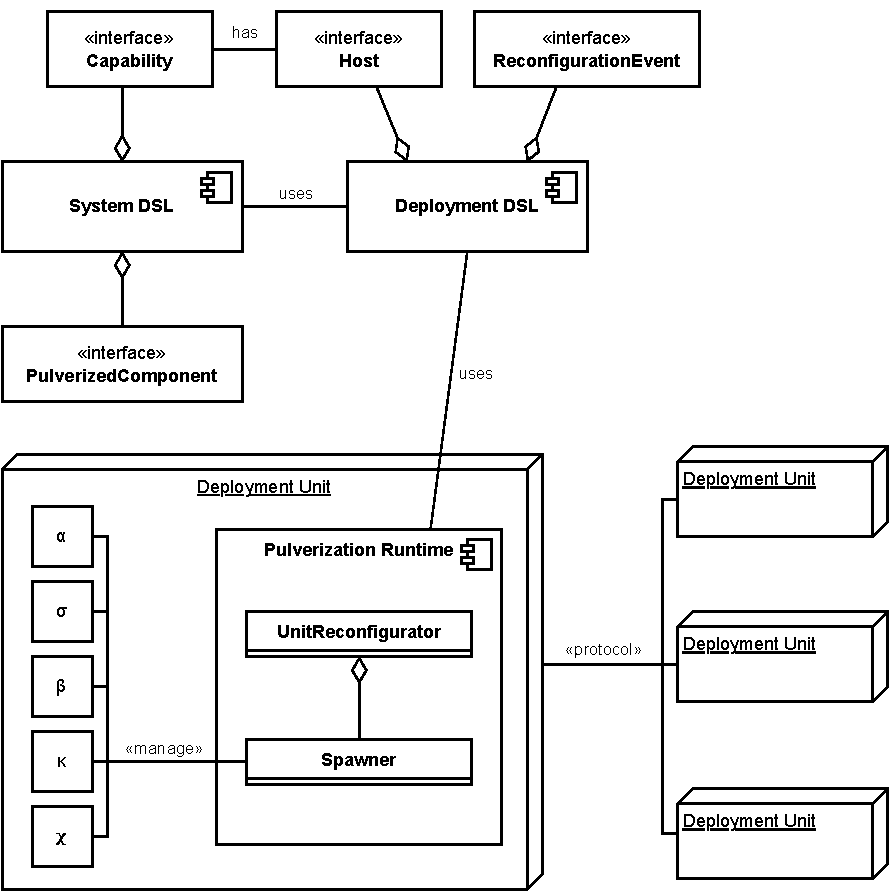
\includegraphics[width=\columnwidth]{figures/pulverization-framework-overview.drawio.pdf}
\caption{The approach provides two \acp{dsl} and a runtime for specifying and executing deployment plans. Each deployment unit will be delivered to the target site and properly configured to interact with other deployment units, as required by the application at hand (see  \Cref{sec:evaluation} for examples).}
\label{fig:approach}
\end{figure}



\subsection{On Middlewares and (Domain-Specific) Languages for Deployed Systems Specification and Execution}
\label{sec:contrib:general}

As mentioned in \Cref{sec:background:dep},
 the deployment and re-configuration of a software system
 may be supported -- following the well-known layered architectural style -- by a \emph{runtime} or \emph{middleware}~\cite{DBLP:journals/cacm/GazisK22}
 encapsulating, among others, deployment and reconfiguration services.
%
The runtime could be reified into a deployment unit \emph{per se},
 or can be implemented as part of the deployment units of the software system to be deployed---e.g., taking the form of an \emph{\ac{api}} or a \emph{framework}.
%
In order to take decisions about deployment and reconfiguration, 
 such a runtime has to be \emph{configured}
 for the software application at hand,
 i.e., it has to be given a \emph{deployment plan} capturing deployment mappings, constraints, and policies.
%

In principle, there are several possibilities to implement a deployment plan:
%
(i) declaratively, through a set of \emph{configuration files};
(ii) through a \emph{\ac{api}/library}, implemented in a general-purpose language;
or 
(iii) through a \ac{dsl}~\cite{dsl-book-voelter}. % configured with its own custom syntax.
%
These approaches have different trade-offs.

A framework/runtime with configuration files enforces declarativity at the configuration level,
but its flexibility is limited,
as options that have not been accounted for at design time can hardly be injected through configuration files.
%
A (well designed) library can be flexible as the host language can be used to express peculiar configurations
and easier to adopt to users acquainted with the host language;
but its configuration may quickly become imperative and harder to maintain as complexity grows.
%
Finally, a \ac{dsl}~\cite{dsl-book-voelter} can be designed to be as expressive as needed,
but it has high maintenance cost (as the language maintenance costs stack upon those of the library/\ac{api}) and, potentially,
a steep learning curve due to the need of learning a new (custom) language.

Recent evolution in programming languages,
however,
open to an additional strategy:
the construction of \emph{internal} \acp{dsl},
hybrids between libraries and stand-alone (external) \acp{dsl}~\cite{dsl-book-voelter}.
%
In fact, modern languages such as Kotlin, Groovy, Ruby, and Scala~\cite{Riti2018}
provide specific syntactic features to enable the construction of APIs whose ergonomy is akin to the one of a dedicated language,
but that are valid fragments in the host language.
%
Although internal \acp{dsl} are de facto libraries in the host programming language
(there is no clear boundary defining when a library becomes a \ac{dsl}\footnote{\url{https://archive.is/wip/xAeiX}}),
from a practical perspective
they allow for great flexibility and ergonomy
(although not total as the one of a custom \ac{dsl}, as they are subject to the syntactic constraints of the host language)
while retaining a reduced maintenance cost
(as the host language ecosystem and tooling can be reused directly)
and a gentle learning curve compared to stand-alone \acp{dsl}
(as the syntax will be largely familiar to the host language users).
%
Compared to external ones
internal \acp{dsl} allow the designer to fall back to the host language directly
to implement peculiar entities or processes that cannot be express by the \ac{dsl}.
%
The approach has thus been successfully applied in several domains,
spanning from
build systems\footnote{\url{https://archive.is/5xtaN}}
and ontologies~\cite{DBLP:journals/jossw/Balhoff16} to
hardware design~\cite{DBLP:journals/trets/SerreP20} to
logic~\cite{2pkt-swx16} and aggregate programming~\cite{DBLP:journals/softx/CasadeiVAP22}.
%

\subsection{The \dslSys{}: Components and Required Capabilities}
\label{sec:contrib:dslsys}

The \dslSys{} captures the concepts of
\emph{device type}, \emph{component}, \emph{capability}, and \emph{requirement}.
%
A reference sample is presented in \Cref{lst:system-configuration}.
%
The DSL provides simple means to define capabilities as types in the host language (Lines~\ref{capab:start}--\ref{capab:end}),
and then to associate them to pulverised components for each device type (Lines~\ref{devcap:start}--\ref{devcap:end}).
%
This \ac{dsl} is meant to define constraints that the application imposes on the infrastructure,
ruling out configurations that are not capable to support the system
(for instance, deploying the sensor component of a device in a host that exposes no sensor).
%
All combinations of components and capabilities that are defined as supported become instead amenable as \emph{targets} of deployment or reconfiguration---forming what we may call the \emph{deployment range}.
%\emph{runtime reconfiguration}.
%
In the example, e.g., component \texttt{Behavior} in \texttt{iot-sensor} is defined as executable on any of host exposing
\texttt{HighCPU} and/or \texttt{EmbeddedDevice} as capabilities (\Cref{devcap:b}):
it implies that the component can be dynamically moved to any host offering any such capability.

%\lstinputlisting[
%    float=ht,
%    language=Kotlin,
%    caption={
%        Example infrastructure configuration,
%        defining three capabilities and a system composed of two device types,
%        each component of which is then bound to the set of capabilities it needs to execute.
%    },
%    label=lst:system-configuration,
%]{listings/SystemConfig.kt}

\begin{lstlisting}[
    float=ht,
    language=pulv,
    caption={
        Example of \dslSys{} usage.
        This code snippet defines three capabilities and a logical system composed of two device types,
        whose components are bound to the set of capabilities they needs to execute.
    },
    label=lst:system-configuration,
    escapechar=\%,
    numbers=left
]
object HighCPU : Capability%\label{capab:start}%
object LowLatencyComm : Capability
object EmbeddedDevice : Capability%\label{capab:end}%

val conf = pulverizedSystem {
  device("control-center") {%\label{devcap:start}%
    Behavior and State deployableOn HighCPU
    Communication deployableOn LowLatencyComm
    Sensors deployableOn EmbeddedDevice
  }
  device("iot-sensor") {
    Behavior deployableOn setOf(HighCPU, EmbeddedDevice)%\label{devcap:b}%
    Communication deployableOn LowLatencyComm
    Sensors and Actuators deployableOn EmbeddedDevice
  }%\label{devcap:end}%
}
\end{lstlisting}


\subsection{The \dslDep{}: Deployment Domain, Mapping, and Reconfiguration}
\label{sec:contrib:dsldep}

The \dslDep{} supports the definition of the mapping between pulverised components and specific hosts,
as well as the definition of reactive reconfiguration policies.
%
It works with the concepts of \texttt{Host}
(associated to \texttt{Capability}),
\texttt{ReconfigurationEvent},
and \texttt{ReconfigurationRule}.
%
Using \Cref{lst:runtime-configuration} as a reference example,
we show how reconfiguration events (Lines~\ref{code:reconfigev:start}--\ref{code:reconfigev:end}) can be captured at the type-system level
by expressing them as a predicate over an asynchronous flow of \texttt{events} influencing the system's state.
%
Similarly, hosts can be configured by defining their name and capabilities (Lines~\ref{code:hosts:start}--\ref{code:hosts:end}).
%
Once the hosts composing the system have been configured,
the entire infrastructure can be set up (Lines~\ref{code:infra:start}--\ref{code:infra:end}) by defining,
for each logical device,
which host should host each pulverised component (Lines~\ref{code:mapping:start}--\ref{code:mapping:end}).
%
Additionally,
reconfiguration rules (Lines~\ref{code:reconfig:start}--\ref{code:reconfig:end}) can be defined to specify how the system should react to reconfiguration events.
%
In this context, the \ac{dsl} exposes a special syntax to express the migration of a pulverised component on a different host.
%
Crucially, being the DSL internal,
specialised behaviour not supported by the \ac{dsl} can be defined in the host language directly:
configuration blocks surrounded by curly brackets are,
in fact,
plain lambda expressions, supporting any kind of computation.

\makeatletter
\newcommand\currentStyle@lstparam{}
\lst@AddToHook{Output}{\global\let\currentStyle@lstparam\lst@thestyle}
\lst@AddToHook{OutputOther}{\global\let\currentStyle@lstparam\lst@thestyle}
\makeatother

\makeatletter
\newcommand{\crefe}[1]{\currentStyle@lstparam\Cref{#1}} %<-- try to change that to `xs'
\makeatother

\begin{lstlisting}[
    float=ht,
    numbers=left,
    language=pulv,
    caption={
        Example of the usage of the domain-specific language for the runtime configuration.
        The example defines the runtime configuration of the system, specifying the initial deployment and the reconfiguration rules.
    },
    label=lst:runtime-configuration,
    numbers=left,
    escapechar=\%
]
// Reconfiguration events %\label{code:reconfigev:start}%
expect fun cpuLoad(): Flow<Double>
expect fun batteryLevel(): Flow<Double>
object HighLoad : ReconfigurationEvent<Double>() {
  override val predicate = { it > 0.90 }
  override val events = cpuLoad()
}
object LowBattery : ReconfigurationEvent<Double>() {
  override val predicate = { it < 0.20 }
  override val events = batteryLevel()
}%\label{code:reconfigev:end}%
// Available hosts %\label{code:hosts:start}%
object Smartphone : Host {
  override val hostname = "smartphone"
  override val capabilities = setOf(EmbeddedDevice)
}
object Server : Host {
  override val hostname = "amazon-aws"
  override val capabilities=setOf(HighCPU,LowLatencyComm)
}%\label{code:hosts:end}%
// Runtime initial setup and runtime reconfiguration rules %\label{code:infra:start}%
val infrastructure = setOf(Smartphone, Server)
val conf = // see %\crefe{lst:system-configuration}%
pulverizationRuntime(conf, "iot-sensor", infrastructure) {
  DeviceBehaviour() startsOn Server%\label{code:mapping:start}%
  DeviceCommunication() startsOn Server
  DeviceSensors() startsOn Smartphone
  DeviceActuators() startsOn Smartphone%\label{code:mapping:end}%
  reconfigurationRules {%\label{code:reconfig:start}%
    onDevice {
      HighLoad reconfigures {Behaviour movesTo Smartphone}
      LowBattery reconfigures {Behaviour movesTo Server}
    }
  }%\label{code:reconfig:end}%
}%\label{code:infra:end}%
pulverizationRuntime(conf, "control-center", infrastructure) {
  /* ... */
}
\end{lstlisting}

% A \texttt{ReconfigurationEvent} is characterized by the \emph{events}
% that it produces and the \emph{condition} that must be satisfied to trigger the reconfiguration.
% %
% The \emph{events} are represented as an asyncronous stream of valued produced by the device and the
% \emph{condition} is a predicate that is evaluated on the stream of events.
% %
% At the first match of the condition, the reconfiguration is triggered and the system is reconfigured with the new deployment.
% %
% The~\Cref{lst:reconfiguration-events} shows an example of the definition of a reconfiguration event.

% \lstinputlisting[
%     float=ht,
%     language=Kotlin,
%     caption={Example of the definition of a reconfiguration event.},
%     label=lst:reconfiguration-events,
% ]{listings/ReconfigurationEvents.kt}

\subsection{Implementation details and underlying runtime}
\label{sec:contrib:runtime}

We implemented the proposed \ac{dsl} in Kotlin.
%
We wanted a language with a strongly typed syntax to help developers with better contextual assist,
and we wanted the possibility to target multiple runtimes
(Kotlin currently targets the JVM, JavaScript, and native code for many platforms\footnote{\url{https://archive.is/JSiTg}},
including mobile and wearable devices)
and be as interoperable as possible with other languages.
%
Scala could have been a good alternative,
but we deemed the multiplatform support of Kotlin a better fit for our needs.
%
The framework has been open sourced and released with a permissive license\footnote{\url{https://github.com/pulvreakt/pulvreakt}}.

The runtime bases its operation on three main components:
the \texttt{Spawner}, which is responsible for executing the components;
the \texttt{UnitReconfigurator}, which is responsible for reconfigure the \emph{deployment unit}
according to the \texttt{ReconfigurationEvent}
and the \texttt{Communicator}s which are used to establish the components' intra-communication.
%
To start, the \texttt{PulverisationRuntime} needs to know the name of the \emph{logical device},
the \emph{host} on which is running, and the configurations produced by the two \ac{dsl}s.
%
At the start of the system the runtime,
based on the provided configuration,
spawns all the components that must start on the \emph{deployment unit}.
%
Similarly, the \texttt{UnitReconfigurator} starts observing all the configured \texttt{ReconfigurationEvent}s,
and registers the listeners for incoming reconfigurations.
%
Each spawned component starts to execute its logic and shares data with other component via the \texttt{Communicator},
which is responsible for the components' intra-communication by leveraging the communication protocol.
%
When a reconfiguration occurs, the \texttt{UnitReconfigurator} takes into account the new deployment configuration,
by interacting with the \texttt{Spawner}, to start or stop the required components.

The configuration produced by the \ac{dsl} needs a platform that instructs the system on the way actual communication needs to be performed.
%
In our current implementation,
we provide out of the box a JVM platform based on the AMQP protocol leveraging RabbitMQ,
supporting both intra- and inter-device communication.
%
The platform also features an optimisation for pulverised components of the same logical device ending up running on the same host:
as it would be expected,
they would communicate directly by sharing memory,
without the need to go through (de)serialisation processes and networking.
%
For the large scale experiment,
we implemented a second platform,
this time to comply with the requirements of the simulation engine we used.
%
The implementation required little effort,
and it has been made available as part of the evaluation repositories.

\section{Evaluation}\label{sec:evaluation}

In this section,
we exercise the proposed framework through two case studies.
%
In the former,
we show a small-scale demonstrator of a safety system warning people when a room capacity is exceeded,
to showcase the integration of the framework with established technologies\footnote{
    \url{https://github.com/nicolasfara/ACSOS-2023-pulverization-crowd-room}
};
in the latter,
we simulate a city-scale distributed application deployed for a urban event
and show how the dynamic reconfiguration may help achieving balance between energy consumption and \ac{qos}\footnote{
    \url{https://github.com/nicolasfara/ACSOS-2023-pulverization-evaluation}
}.
%
Both experiments have been released with a permissive open-source license and have been archived for future reference on
Zenodo~\cite{https://doi.org/10.5281/zenodo.7933160, https://doi.org/10.5281/zenodo.7948801}.

\subsection{Small scale: crowd alert}
\label{sec:small-scale-crowd-alert}

In this example, we exercise the framework on a real-world testbed
located in a laboratory.
%
In particular,
we want to avoid situations in which too many people are too close to each other in the same room for safety reasons.
%
To do so,
we equip each person with a wearable device that is able to detect the distance from other similar devices via Bluetooth.
%
For the sake of simplicity,
in the experiment we relied on smartphones to emulate wearables,
and we used
% \meta{
%     NICOLAS please write here (within meta, so that it remains blue)
%     what you used to measure the signal strenght and estimate the distance.
%     Even formulas, calibration procedures, and stuff
% }
%
%\meta{
    the Bluetooth \ac{rssi} to estimate the distance $d$ between devices as:
    $$d=10^{\frac{R_{ref} - R}{10 \cdot n}}$$
    where $R_{ref}$ is the \ac{rssi} reference value at 1 meter
%    (calibrated in a test environment by measuring it with two smartphones),
    R is the currently measured \ac{rssi},
    and $n$ is the path loss exponent,
    a parameter indicating the rate at which the \ac{rssi} decreases with distance.
    %
    $R_{ref}$ and $n$ are environment-sensitive parameters that require calibration;
    we set up a test with two smartphones and measured,
    for our setup,
    $R_{ref}\qty{-60}{\decibelmeter}$ and $n=\qty{2.0}{\decibel}$.
%    Since the definition of $A'$ and $n$ is not trivial,
%    and depends on the environment in which the system is deployed,
%    we have calibrated the system in a test environment by measuring the RSSI signal
%    at 1 meter using two smartphones.
%    %
%    The following values emerged from the calibration phase:
%    $A=\qty{-60}{\decibelmeter}$ and $n = \qty{2.0}{\decibel}$.
%}
%
We used a monitor to issue the warning
by setting its colour from green to red depending on the average distance among people:
the shorter the distance, the redder the tone.
%
\Cref{fig:crowd-alert} shows a representation of the scenario.
%
\begin{figure}
    \centering
    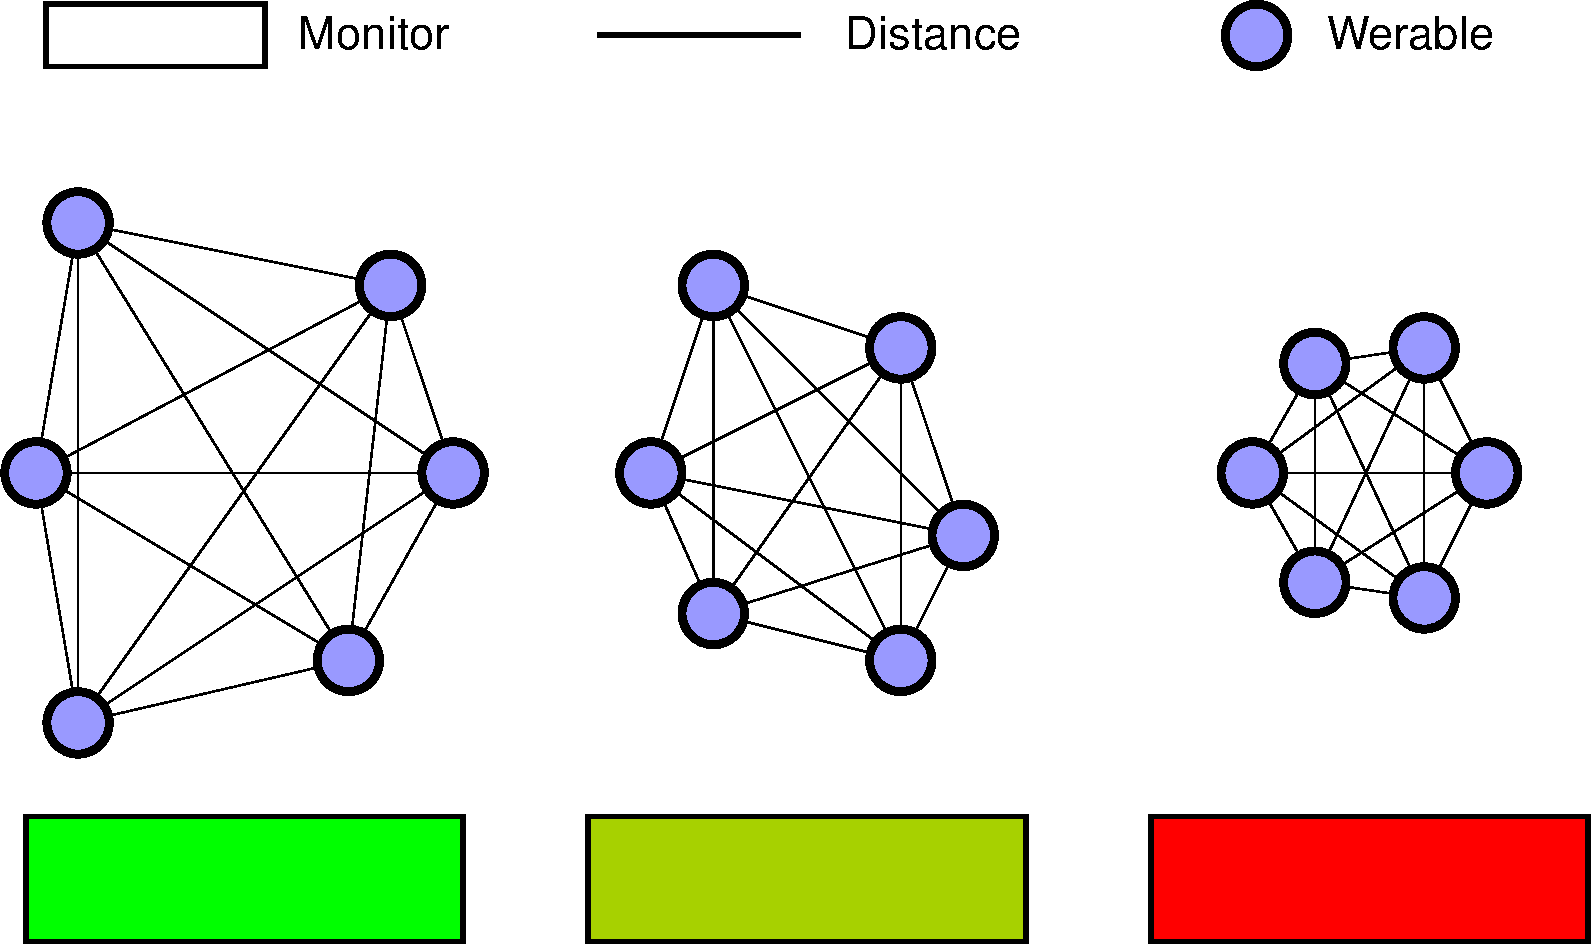
\includegraphics[width=.9\columnwidth]{figures/crow-laboratory-demo.drawio.pdf}
    \caption{
        Representation of the scenario described in \Cref{sec:small-scale-crowd-alert}.
        graph dots represent wearables,
        and arcs lenghts represent the distance between them.
        %
        The rectangle at the bottom represents the monitor.
        %
        The closer the wearables are, the higher is the alert level
        (reddish tones).
    }
    \label{fig:crowd-alert}
\end{figure}

The system is composed of two kinds of device: \emph{wearable} and \emph{alert}.
%
Wearables consist of the following pulverised components:
sensors ($\sigma^w$), perceiving other devices by their signal strength;
behaviour ($\beta^w$), converting raw data from the sensor into messages for the alert system; and
communication ($\chi^w$) sending data to the alert system.
%
They do not need state nor actuators.
%
The alert consists of the following pulverized components:
$\beta^a$, computing the mean distance among devices;
$\kappa^a$, storing the distances measured by the device for comparison with the recent past;
%\meta{
%    NICOLAS what does this do? write within this meta block.
%    %
%    Hold in memory the updated distances between the devices.
%};
$\chi^a$, responsible for receiving the data from the wearable devices;
$\alpha^a$, enacting the alarm by showing a color on the screen.
%
It needs no sensors.

We use the following hosts in the scenario:
\begin{itemize}
    \item multiple \emph{Smartphones}, one per user, emulating wearables and used as distance sensors;
    \item a \emph{Monitor} used to show the alarm;
    \item a \emph{Server} used run crowd estimation and wearable logic.
\end{itemize}

Initially, $\beta^{w}$ is allocated to the \emph{Server} while
$\sigma^{w}$ and $\chi^{w}$ are executed on the \emph{Smartphones},
and all the \emph{alert} components are executed in the \emph{Monitor}.
%
In the experiment,
we define a rule by which,
if the \emph{Server} is overloaded,
$\beta^{w}$ is moved to the \emph{Smartphones}
(with each smartphone running the $\beta^{w}$ corresponding to its $\sigma^{w}$).
%
During the experiment,
we launch several heavy-duty processes on the \emph{Server},
and we observe how the system reacts to the overload.
%
We rely on the MQTT platform module for all the communication,
meaning that both intra- and inter-device communication is handled by the same protocol and broker.

As soon as the reconfiguration event is triggered,
the $\beta$ component of the \emph{Wearable} is moved from the \emph{Server} to the \emph{Smartphone} $s$ hosting $\sigma^{w}_{s}$,
relieving the server and preserving while retaining the system in nominal conditions.
%
The reconfiguration of the system in entirely managed by the framework,
which handles all the machinery and communication to move the component from
one host to another.

This example has been used as a real-world testbed driving our experimental implementation.
%
For the sake of brevity,
we do not report the entire configuration in this manuscript, but it is available in the companion artifact~\cite{https://doi.org/10.5281/zenodo.7933160}
% \meta{
%     NICOLAS please replace TBD with the artifact citation from zenodo. Use doi2bib to get the bibtex entry.
% }
for those willing to exercise the whole system.
%
To simplify testing we also provide,
in the same artifact,
a simulation of the system where every device is containerized.

\subsection{Large scale: urban event}

To show the potential benefit of automatic reconfiguration in \acp{cas},
we consider a large-scale scenario where a crowd of people is attending an event in a city
to participate in a collective activity whose computational weight is relevant, for instance
a tournament of a geo-located game similar to Ingress\footnote{\url{https://www.ingress.com/}}
or Pokémon Go\footnote{\url{https://pokemongolive.com/}}).
%
We suppose the application to be pulverised,
and its behaviour to be able to run either on the smartphones or in cloud.
%
We assume the event to start with users located in random positions in the city,
and to have a recharging station available at that place.
%
The game requires to physically move in the city,
reach a \ac{poi} and perform some operations once there.
%
We assume users with low battery to turn off the application and move to their start station to recharge the device
before rejoining the game.
%
The application is pulverised and its behaviour can execute either on the device or in the cloud.
%
We configure the framework to move the behaviour to the cloud when the battery level
(measured as a percentage of the maximum charge)
is below a threshold $\lambda$,
and to move it back to the device when the battery is charged enough to cross a threshold $\upsilon$
(stable configuration have $\upsilon{}>\lambda$,
otherwise the system continuously moves the behaviour between cloud and devices).
%
We thus indicate any configuration with $\Updownarrow^{\upsilon}_{\lambda}$,
with the exception of two cases:
$\upsilon, \lambda > 100$, forcing the behaviour to be always in the cloud, that we indicate with $\Uparrow$;
and $\upsilon, \lambda < 0$, forcing the behaviour to be always on the device, that we indicate with $\Downarrow$.
%
We are interested in the following metrics:
%
\begin{itemize}
    \item $P_{devices}$ ($kW$), the average device power consumption, a proxy for the battery life;
    \item $P_{cloud}$ ($kW$), the average power consumption of the cloud, if added to $P_{devices}$
    provides the total power consumption
    (hence, assuming a non-carbon-neutral energy mix, it is also a proxy for the carbon footprint);
    \item Distance ($km$), the total distance walked by the participants, a proxy for the \ac{qos},
    as users that need to stop and recharge stop walking;
    \item $\$_{cloud}$ (\$), the price paid to keep the required cloud instances up and running.
\end{itemize}

\subsubsection{Energy model}

\acrodef{epi}[EPI]{Energy Per Instruction}
\acrodef{tdp}[TDP]{Thermal Design Power}

We assume that the power consumption of the device is linearly dependent on the CPU usage,
and we thus decided to estimate the \ac{epi}~\cite{DBLP:conf/islped/ShaoB13}
of common smartphone ($EPI_{device}$) and server ($EPI_{cloud}$) CPUs.
%
To do so, we take the \ac{tdp} of a
Qualcomm Snapdragon 888 ($5W$)
and an
Intel Xeon Platinum P-8124 ($220W$)
and we divide it by the score the CPU obtained in the popular Passmark benchmark\footnote{\url{https://www.cpubenchmark.net/}}
($9362$ and $22674$, respectively)
obtaining an indication of the power per benchmark point
($\nicefrac{5W}{9362pts}$ and \nicefrac{220W}{22674pts} respectively).
%
We then used these ratios to estimate the relative \ac{epi} of the two CPUs,
obtaining a $EPI_{ratio}$ close to 1:18.
%
Thus,
we take the \ac{epi} estimation for the server CPU from~\cite{DBLP:conf/islped/ShaoB13},
(approximately 10J per instruction, considering 36 logical cores of our reference processor)
and we assume the \ac{epi} of the smartphone CPU to be 18 times lower.
%
Once the \acp{epi} of the two platforms are known,
we estimate the number of instructions of the pulverised components as follows:
we assume the application to be a heavy-duty game,
capable to drain the battery of a smartphone
(approximately 4500mAh in capacity, and thus, at 3.3V, 14.85Wh, 53460J)
in 6 hours of continuous usage,
which divided by the \ac{epi} of the smartphone CPU gives us the number of instructions.
%
Additionally,
we account for a variable quota of instructions that captures other activities of the devices
(screen, operating system, other applications, etc.).

\subsubsection{Cost model}
We assume the cloud to be composed by a set of Amazon \emph{AWS} instances,
specifically, \emph{m5.16xlarge} instances
(using our reference server CPU)
the \emph{AWS}
with a hourly cost of \$3.584\footnote{\url{https://aws.amazon.com/ec2/pricing/on-demand/}}
%
We estimate the number of instances required to run the pulverised components by
dividing the total power consumption of the cloud by the \ac{tdp} of the server,
assuming the CPU to be the dominant energy consumption component,
and assuming that each vCPU on AWS maps to a logical core of the underlying hardware.

\subsubsection{Implementation}
We implemented our simulations by interfacing \ourframework{}
with the Alchemist Simulator~\cite{PianiniJOS2013}
through a dedicated platform module.
%
We ran experiments varying the number of participants (hence, smartphones): 100, 300, and 1000
and the \ourframework{} reconfiguration rules:
$\Uparrow$ (behaviour always in the smartphones),
$\Updownarrow^{60}_{20}$,
$\Updownarrow^{80}_{20}$,
$\Updownarrow^{60}_{40}$,
$\Updownarrow^{80}_{40}$,
$\Downarrow$ (behaviour always in the cloud).
%
All the hybrid configurations
(all except $\Uparrow$ and $\Downarrow$)
require runtime reconfiguration to be realised.
%
For each experiment, we run a total of 10 repetitions with a different random seed;
all results are averaged over them.
%
The experiment has been open sourced
and the code has been archived on Zenodo~\cite{https://doi.org/10.5281/zenodo.7948801}.
%
\begin{figure}
    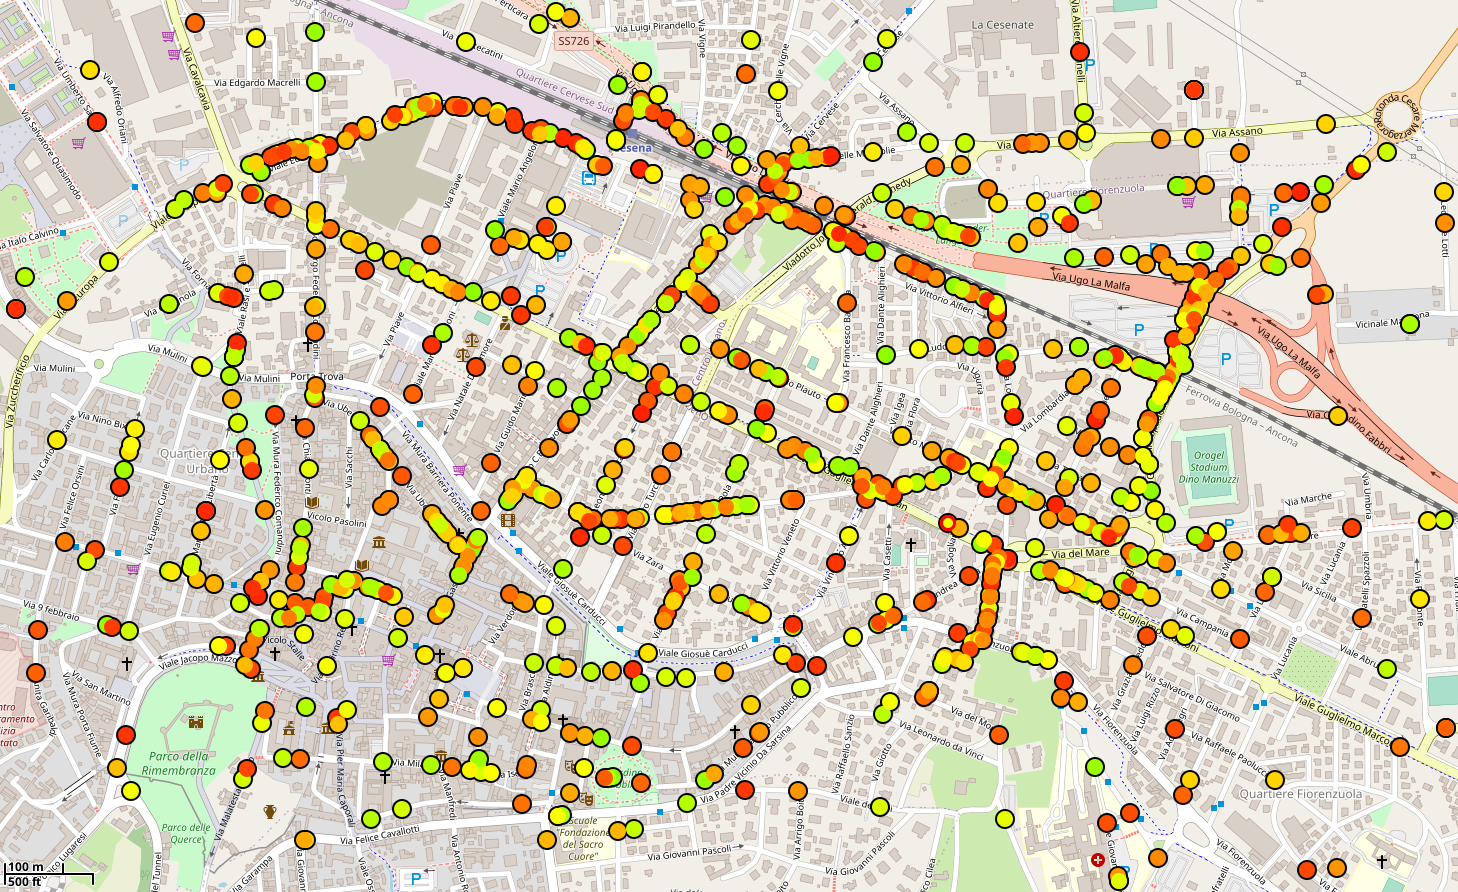
\includegraphics[width=\linewidth]{figures/simulation-screenshot.png}
    \caption{
        A snapshot of the large-scale simulation.
        Smartphones are represented as coloured circles,
        with the color indicating their battery level
        (green when charged, red when low).
    }
    \label{fig:simulation-screenshot}
\end{figure}
%
\Cref{fig:simulation-screenshot} shows a snapshot of the simulation


\subsubsection{Results}
%
\begin{figure}
    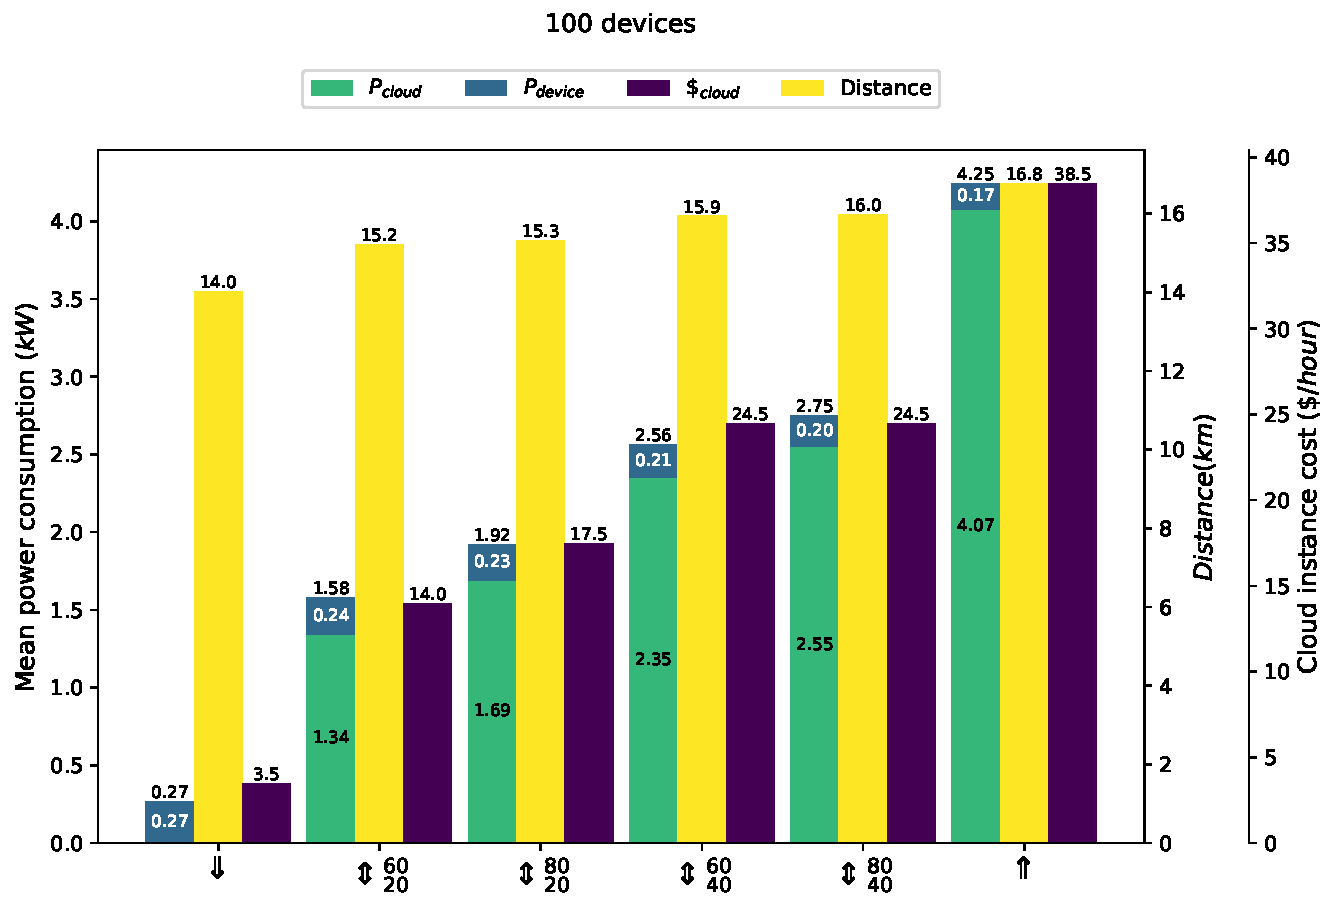
\includegraphics[width=\columnwidth]{figures/cloud_cost-device_consumption-cloud_consumption-distance-device=100.0.pdf}\\
    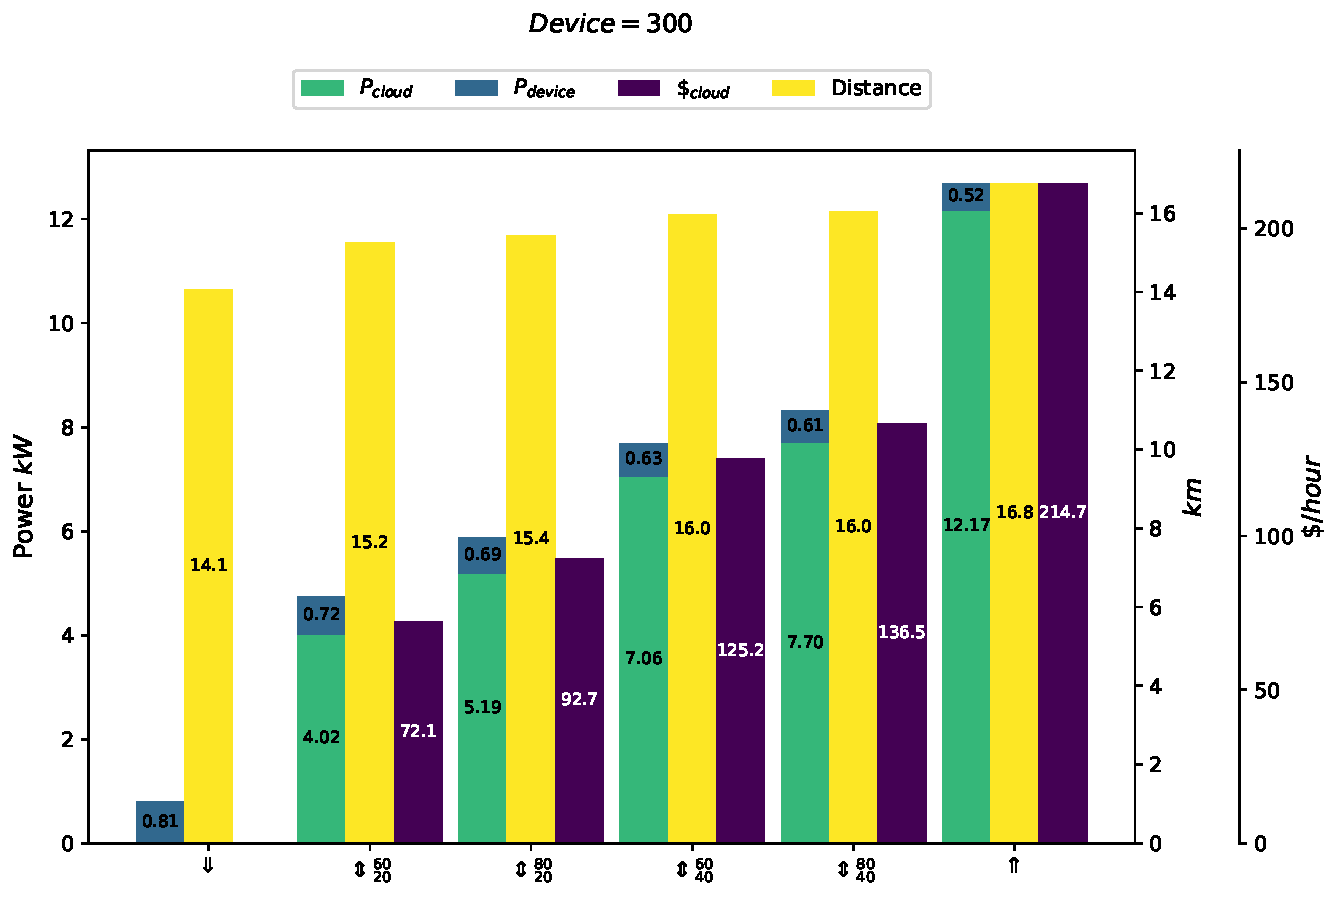
\includegraphics[width=\columnwidth]{figures/cloud_cost-device_consumption-cloud_consumption-distance-device=300.0.pdf}\\
    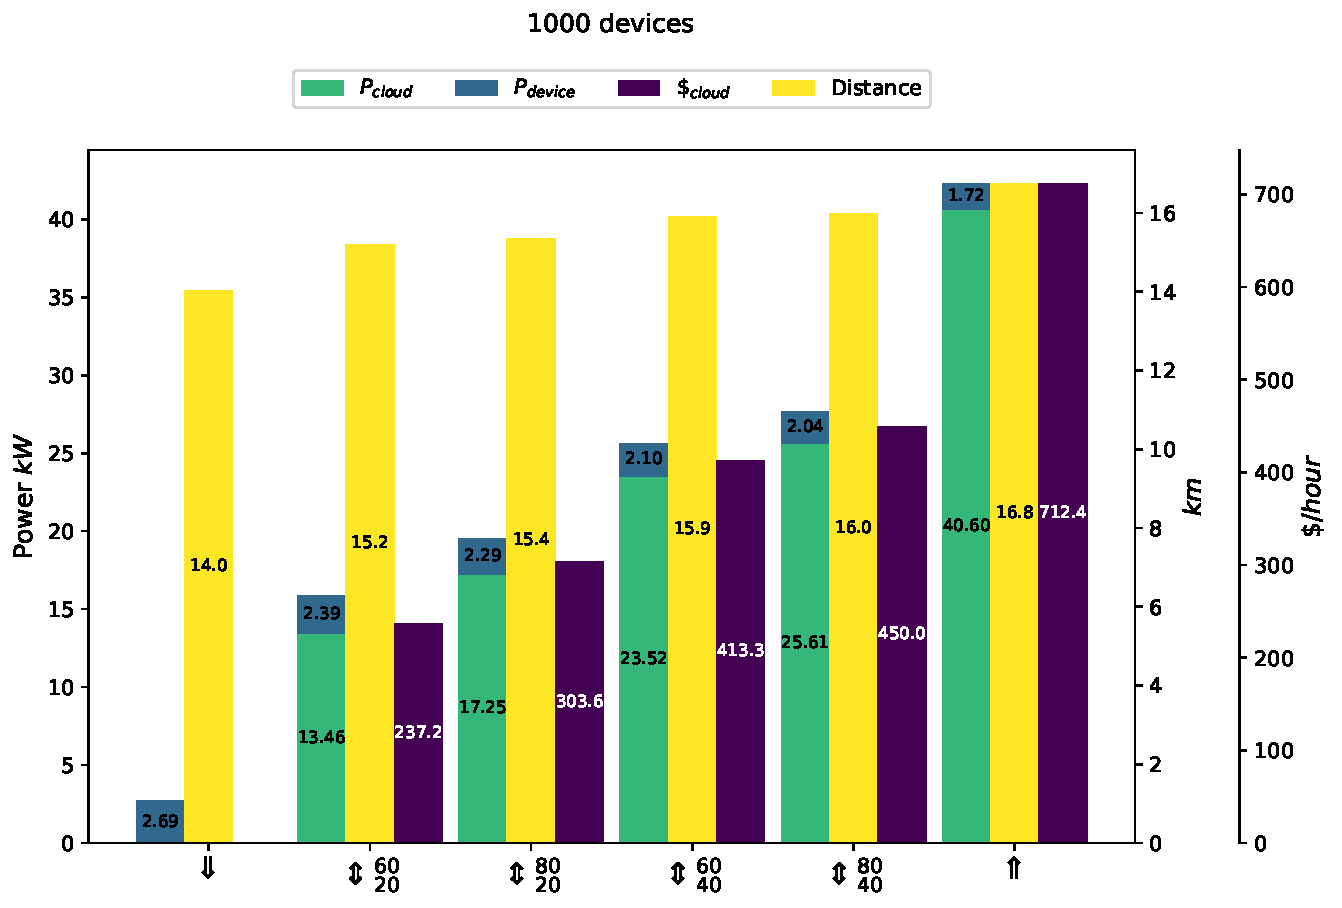
\includegraphics[width=\columnwidth]{figures/cloud_cost-device_consumption-cloud_consumption-distance-device=1000.0.pdf}
    \caption{
        Simulation results for 100 (top), 300 (center), and 1000 (bottom) devices;
        showing all four metrics:
        $P_{cloud}$ ($kW$) in green,
        $P_{devices}$ ($kW$) in blue,
        Distance in yellow, $\$_{cloud}$ in dark purple.
        %
        $P_{cloud}$ and $P_{devices}$ are stacked to also show the overall power consumption.
        %
        Different reconfiguration rules are indicated on the horizontal axis.
        %
        Runtime reconfiguration of the deployment opens to more opportunities to find the trade-off of cost,
        energy use, and \ac{qos} that best fits the current context.
    }
    \label{fig:results}
\end{figure}
%
Results are summarised in \Cref{fig:results}.
%
$\Downarrow$ has the worst \ac{qos}, but also the lowest cloud cost and overall energy consumption.
%
Opposedly, $\Uparrow$ improves the \ac{qos}, but costs and energy use grow significantly.
%
The ability to reconfigure the deployment at runtime
by moving the behaviour from the cloud to the smartphones and vice versa
depending on the battery level allows to find different trade-offs between these two extremes.

\section{Related Work}
\label{sec:rw}

%This work provides 
% \acp{dsl}
% for specifying 
% distributed systems (partitioned according to the 
% pulverisation model)
% and
% corresponding deployment plans,
% and a framework for executing
% deployment plans and reconfigurations.
%
Following the conceptual framework introduced in \Cref{sec:background:dep},
 in this section we cover related work about
 languages for 
 specifying distributed systems (\Cref{sec:rw:whatsw}),
 languages for specifying infrastructures and deployments (\Cref{sec:rw:depdesc}),
 and
 techniques for automatic deployment and reconfiguration (\Cref{sec:rw:autodep}).
 
 
 
\subsection{Application description languages: component-based software engineering and the pulverisation model}
\label{sec:rw:whatsw}
%
%% A first distinction revolves around whether 
%% the distributed software to be deployed 
%% is a monolith 
%% or is already broken into different components.
%
We consider a distributed application 
 as a graph of deployable units.
%
This partitioning may be 
 manually specified at development time
 (e.g., by explicitly defining and packaging different components)
 or automatically defined
 through \emph{application partitioning} approaches~\cite{DBLP:journals/jnca/LiuASGBQ15}. %exploiting the natural modularity of code (depending on the paradigm and language adopted).
 
In our approach, the application partitioning into components is manually specified through a \ac{dsl}.
%
Therefore, it can be framed in the context of \emph{component-based software engineering},
 with ~\cite{vale2016component-based-se} providing a comprehensive review.
%
The specification or design of distributed systems
 may leverage
 component models~\cite{DBLP:journals/tse/CrnkovicSVC11},
 architectural description languages~\cite{DBLP:journals/tse/MedvidovicT00},
 service-based compositions~\cite{DBLP:journals/csur/LemosDB16}, 
 or frameworks.
%
Specifically,
 this work builds on the \emph{pulverisation} component model~\cite{FI2020-pulverization,IEEE-IoTJ-pulverization-simulation}.
 whereby a large-scale cyber-physical system
 is partitioned into a graph of devices
 where each device is split into five deployable components:
 (i) sensors interface,
 (ii) actuators interface,
 (iii) behaviour,
 (iv) state, and
 (v) communication component.
%
In~\cite{IEEE-IoTJ-pulverization-simulation},
 a methodology on top of the pulverisation model
 is proposed
 for generating and testing deployments through simulation.

Additionally,
 the approach of specifying in a single codebase 
 parts of the structure, behaviour, and/or interaction 
 for a whole distributed system
 is also related to \emph{macroprogramming}~\cite{Casadei2023macro}
 and, in particular, to \emph{multi-tier programming} paradigm~\cite{DBLP:journals/csur/WeisenburgerWS20},
 where the deployment units for different tiers
(e.g., client and server tiers; or view, business logic, and data tiers)
are obtained by compilation or interpretation of a single codebase.

\subsection{Infrastructure and deployment description languages}
\label{sec:rw:depdesc}

A \emph{deployment plan} is a configured mapping of a software system onto a deployment domain.
%
Given a deployable software system
developed using the techniques of the previous subsection,
 what is needed now is a language to describe a deployment domain
 and the deployment mapping.
%
Languages have been proposed
 targeting specific kinds of deployment domains
 such as the smart grid (cf. \emph{dspec} in the \emph{RIAPS} platform~\cite{DBLP:conf/coins/GhoshTKKL22})
 or the cloud (cf. the \emph{CAMEL} multi-\ac{dsl}~\cite{DBLP:journals/jcloudc/AchilleosKRKDOS19}).

In this work,
 we are especially interested in deployments over large-scale cyber-physical systems and the edge-cloud continuum.
%
\emph{MuScADeL}~\cite{DBLP:conf/compsac/BoujbelRLTAL14/muscadel}
 is a \ac{dsl} that allows to express deployment properties of 
applications on multi-scale deployment domains,
i.e., large and heterogeneous infrastructures considered under several viewpoints
(device, geography, network, administrative domains, etc.).
%
In~\cite{DBLP:journals/sosym/SongDFSF22},
  a model-based deployment approach is proposed
  targeting so-called \emph{fleets}, i.e.,
  distributed and heterogeneous devices at the edge characterised by different cyber-physical contexts
(cf. resources, connectivity, etc.).
%
It is based on the \emph{GeneSIS} modelling language,
where a \texttt{DeploymentModel} consists of sets of \texttt{Resources} (e.g., \texttt{Component}s, specialised by \texttt{InfrastructureComponent}s and \texttt{SoftwareComponent}s) with associated \texttt{Property}s and \texttt{Link}s.

\subsection{Automatic/autonomic deployment and reconfiguration}
\label{sec:rw:autodep}
%
A comprehensive conceptual framework
 on automatic deployment of distributed systems
 is provided in~\cite{DBLP:journals/jss/ArcangeliBL15}.
%
A more recent survey~\cite{coullon2023swreconfig} focuses
 on formal techniques for verifying the correctness of reconfigurations
 in component-based distributed software systems.
%
Two formal models for specifying reconfigurable architectures are
\emph{DR-BIP}~\cite{Ballouli18dr-bip}
and \emph{DReAM}~\cite{denicola2020dream-dynamic-reconfig-arch-modelling}.
%
Both are based on the same conceptual model: they 
 feature \emph{components} (capturing behaviour),
\emph{connectors} (capturing interaction between components' \emph{ports}),
\emph{maps} (logical topologies),
and \emph{deployments} (associating components to map locations),
overall organised in \emph{motifs} (dynamic architectural configurations),
to model and analyse dynamic architectures.
%
%\meta{TODO: say something about our positioning wrt verification of reconfigurations}

In the \emph{osmotic computing} approach~\cite{DBLP:journals/computer/VillariFDRJR19},
 microservices (the solvent)
 can migrate across 
 the edge-cloud infrastructure (the solution),
 passing through layer boundaries (the semi-permeable membranes),
 in order to keep a balance in the desired properties (the solute).
%
\emph{ASSL}~\cite{DBLP:conf/birthday/VassevH97}
 supports the specification
 of autonomic elements,
 interaction protocols,
 and \emph{self-management policies} based on fluents (states), events, and actions.
%
%In \emph{ConfSolve}~\cite{DBLP:conf/saso/HewsonAG13},
% the language supports the specification of logical \emph{reconfiguration constraints}, which are then solved as a constraint satisfaction problem.
%
The \emph{AWaRE DSL}~\cite{DBLP:conf/aswec/ChhetriLUVKNR18/adsl} supports constraint-based self-management,
leveraging managing agents.
The language enables the specification of the domain model (in terms of components),
the problem structure model (in terms of constraints),
the agent architecture model (in terms of agents, roles, and their coordination), and the assignment model (in terms of management problem assignment strategies).
%
Similar, earlier approaches based on the specification of \emph{constraint-sets} include \emph{DELADAS}~\cite{Dearle2004deladas}
and \emph{ConfSolve}~\cite{DBLP:conf/saso/HewsonAG13}.
%
\emph{Ctrl-F}~\cite{DBLP:journals/jss/AlvaresRS17}
 is an architectural description language
 with constructs for specifying adaptive behaviour 
 and policies (constraints) for the reconfiguration of system components.
%
These approaches, however, typically suffer from scalability issues.

%%high-level constructs to describe adaptation in software components by means of behavioural programs, i.e., in terms of order and/or conditions under which reconfigurations take place; and policies, i.e., constraints that have to be enforced all along the execution. In other words, Ctrl-Fis a first-class language that is applicable to any Component-based application requiring self-adaptation with formal guarantees.
 
 

%\meta{
%MuScADeL (Multi-Scale Autonomic Deployment Language)~\cite{DBLP:conf/compsac/BoujbelRLTAL14/muscadel}
%
%ADSL (AWaRE DSL)~\cite{DBLP:conf/aswec/ChhetriLUVKNR18/adsl} % and see corresp RW: the most related DSLs are those in the area of automated deployment [17]. Such DSLs include Deladas [31], [32], ConfSolve [15], [33], j-ASD’s DSL [34] and MuScADeL [35], [36].DBLP:journals/jss/AlvaresRS17
%% [17]: J.-P. Arcangeli, R. Boujbel, and S. Leriche, "Automatic deployment of distributed software systems: Definitions and state of the art," Journal of Systems and Software, vol. 103, pp. 198–218, 2015
%%
%%%
%%%\subsection{Approaches to Deployment Independence}
%%%\label{s:rw:deployment-independence}
%%%
%%%\meta{TODO: add works on deployment independence, e.g., osmotic~\citep{DBLP:journals/computer/VillariFDRJR19}, BIP~\citep{lekidis2015bip-wsn,bastarrica2001optimization-techniques-deployment-components-bip}}
%%%
%%%We highlight a number of representatieve research efforts on deployment and automatic reconfiguration of systems.
%%%%
%%%%For instance, 
%%%\emph{Osmotic computing}~\cite{DBLP:journals/computer/VillariFDRJR19} is an approach to opportunistic deployment of microservices on the edge-fog-cloud platform.
%%%An osmotic platform aims to reach and maintain an ``osmotic equilibrium'' 
%%%between infrastructural and application requirements
%%%by automatically migrating microservices to deployment locations.
%%%
%%However, the approach mainly targets centrally orchestrated systems.
%%%
%%Other approaches leverage component-based, architectural descriptions to decouple application logic and deployment.
%%%
%%For instance, \emph{DR-BIP (Dynamically Reconfigurable - Behaviour Interaction Priority model)}~\cite{,Ballouli18dr-bip}
%%and \emph{DReAM (Dynamically Reconfigurable Architectural Modelling)}~\cite{denicola2020dream-dynamic-reconfig-arch-modelling}
%%use \emph{components} (capturing behaviour), \emph{connectors} (capturing interaction between components' \emph{ports}), 
%%\emph{maps} (logical topologies),
%%and \emph{deployments} (associating components to map locations),
%%overall organised in \emph{motifs} (dynamic architectural configurations),
%%to model and analyse dynamic architectures.
%%%
%%
%%These approaches have some similarity with the approach presented in this paper, but they are arguably more complex and our  
%%%than the one introduced in this paper,
%% %, though also fostering an exogenous, declarative (logics-based) modelling approach.
%%approach explicitly addresses self-organising CPS.
%%%
%%%
%%%By constrast, our approach explicitly addresses self-organising CPS.
%%%
%%%A more in-depth, formal comparison is left as future work.
%}

\section{Conclusion and future work}\label{sec:conclusion}

In this work we presented a practical \ac{dsl} and framework for the
runtime re-configuration of pulverised \ac{cas} applications.
%
The original idea of pulverisation was to define applications considering arbitrary networks of logical devices,
decompose (pulverise) these logical devices into small deployment units,
and then define their desired deployment at a later time.
%
Through the specialised \ac{dsl} introduced in this work
we have shown that this idea can be realised in practice.
%
Moreover, we extended the original idea of pulverisation with the possibility to specify runtime re-configuration policies,
which can be leveraged to achieve better trade-offs in terms of performance, cost, and resource usage.
%
We provide a real-world demonstrator for the technology,
and we show via simulation that the approach can be beneficial.

In its current form, the proposed \ac{dsl} has two limitations that will be addressed in the future.
%
First and foremost, it currently does not consider openness,
as hosts get specified in the runtime and reconfiguration \acp{dsl} as a closed set.
%
The second limitation is related to the policies that can be expressed in the reconfiguration \ac{dsl}:
currently, only policies that can be assessed at the local host level can be assessed.
%
A policy that requires to consider the state of multiple hosts would require to resort to the host language primitive mechanisms and make explicit communications outside the framework,
thus breaking the abstraction.
%
This limitation can be addressed by extending the current reconfiguration
block of the \ac{dsl} in such a way that queries can be performed on any reachable host of the system,
thus making all communications
(including reconfiguration-related ones)
pass through the channels controlled by the framework.
%
Concurrently with these extensions,
we intend to add support for additional network protocols to be able to support a larger number of practical scenarios.

\bibliographystyle{IEEEtranDOI}
\bibliography{bibliography}

%\vspace{12pt}
%\color{red}
%IEEE conference templates contain guidance text for composing and formatting conference papers. Please ensure that all template text is removed from your conference paper prior to submission to the conference. Failure to remove the template text from your paper may result in your paper not being published.

\end{document}
